\documentclass[10pt,aspectratio=169,serif,fleqn]{beamer}

\usepackage[fontset=none, scheme=plain]{ctex}
\IfFontExistsTF{Songti SC}{%
	\setCJKmainfont{Songti SC}[AutoFakeSlant=0.2]%
	\setCJKsansfont{Songti SC}[AutoFakeSlant=0.2]%
}{%
	\setCJKmainfont{FandolSong-Regular}[Extension=.otf,BoldFont=FandolSong-Bold,AutoFakeSlant=0.2]%
	\setCJKsansfont{FandolSong-Regular}[Extension=.otf,BoldFont=FandolSong-Bold]%
}
\usepackage{amsmath,amssymb,graphicx,tikz,booktabs,multicol,calligra}
\usepackage{pgfplots}
\pgfplotsset{compat=1.18}
\usepackage{tcolorbox}
\tcbuselibrary{skins}
\usepackage{XyygU}
\usepackage{caption}
\captionsetup[figure]{name=图,labelsep=period}

\usetikzlibrary{arrows.meta,positioning,calc}

\setlength{\abovedisplayskip}{0pt plus 2pt minus 2pt}
\setlength{\belowdisplayskip}{0pt plus 2pt minus 2pt}

\title[习题3.4]{习题3.4 \quad 函数的应用（一）}
\subtitle{综合运用 \& 拓广探索}
\author{}
\institute{}
\date{2026-10-16}

\begin{document}

\begin{frame}
  \titlepage
\end{frame}

% ========== 第1题 ==========
\begin{frame}[t]{第1题：汽车往返A、B两地}
\textbf{1.} 某人开汽车以 $60$ km/h 的速率从 $A$ 地到 $150$ km 远处的 $B$ 地，在 $B$ 地停留 $1$ h 后，再以 $50$ km/h 的速率返回 $A$ 地。把汽车与 $A$ 地的距离 $x$（单位：km）表示为时间 $t$（单位：h）（从 $A$ 地出发时开始）的函数；再把车速 $v$（单位：km/h）表示为时间 $t$ 的函数，并分别画出这两个函数的图象。
\end{frame}

\begin{frame}[t]{}
	\vspace{-2em}
\begin{tcolorbox}[colback=orange!10,colframe=orange,title=\textbf{解}]
从 $A$ 到 $B$ 用时 $150/60=2.5$ h，在 $B$ 停留 $1$ h（$t\in[2.5,3.5]$），从 $B$ 返回 $A$ 用时 $150/50=3$ h（$t\in[3.5,6.5]$）。

\vspace{0.3em}
距离 $x(t)$：
\[
x(t)=\begin{cases}
60t, & 0\le t<2.5,\\
150, & 2.5\le t<3.5,\\
150-50(t-3.5), & 3.5\le t\le 6.5.
\end{cases}
\]

\vspace{0.3em}
车速 $v(t)$：
\[
v(t)=\begin{cases}
60, & 0\le t<2.5,\\
0, & 2.5\le t<3.5,\\
-50, & 3.5\le t\le 6.5.
\end{cases}
\]
（返回时速度方向与出发相反，记为 $-50$ km/h）
\end{tcolorbox}
\end{frame}

\begin{frame}[t]{第1题 图象}
\begin{center}
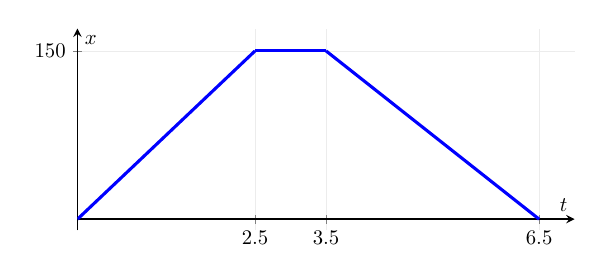
\begin{tikzpicture}[scale=0.75]
\begin{axis}[
    width=10cm, height=5cm,
    axis lines=middle,
    xlabel=$t$, ylabel=$x$,
    xmin=0, xmax=7, ymin=-10, ymax=170,
    xtick={0,2.5,3.5,6.5},
    ytick={150},
    grid=major, grid style={gray!15},
    axis line style={thick},
]
\addplot[line width=1.5pt,blue,domain=0:2.5,samples=2] {60*x};
\addplot[line width=1.5pt,blue,domain=2.5:3.5,samples=2] {150};
\addplot[line width=1.5pt,blue,domain=3.5:6.5,samples=2] {150-50*(x-3.5)};
\end{axis}
\end{tikzpicture}
\quad
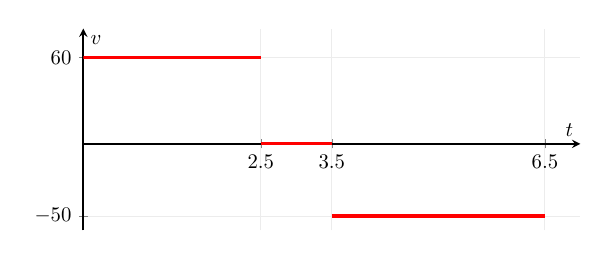
\begin{tikzpicture}[scale=0.75]
\begin{axis}[
    width=10cm, height=5cm,
    axis lines=middle,
    xlabel=$t$, ylabel=$v$,
    xmin=0, xmax=7, ymin=-60, ymax=80,
    xtick={0,2.5,3.5,6.5},
    ytick={-50,0,60},
    grid=major, grid style={gray!15},
    axis line style={thick},
]
\addplot[line width=1.5pt,red,domain=0:2.5,samples=2] {60};
\addplot[line width=1.5pt,red,domain=2.5:3.5,samples=2] {0};
\addplot[line width=1.5pt,red,domain=3.5:6.5,samples=2] {-50};
\end{axis}
\end{tikzpicture}
\end{center}
\end{frame}

% ========== 第2题 ==========
\begin{frame}[t]{第2题：无盖蓄水池造价}
\textbf{2.} 要建造一个容积为 $1200$ m$^3$，深为 $6$ m 的长方体无盖蓄水池，池壁的造价为 $95$ 元/m$^2$，池底的造价为 $135$ 元/m$^2$，如何设计水池的长与宽，才能使水池的总造价控制在 $7$ 万元以内（精确到 $0.1$ m）？
\end{frame}

\begin{frame}[t]{第2题 解答}
	\vspace{-2em}
\begin{tcolorbox}[colback=orange!10,colframe=orange,title=\textbf{解}]
底面积 $S=\dfrac{1200}{6}=200$ m$^2$。设长为 $x$，宽为 $y$，则 $xy=200$。

\vspace{0.3em}
池底造价：$200\times135=27000$ 元。

\vspace{0.3em}
池壁面积：$2\cdot6(x+y)=12(x+y)$，池壁造价：$95\times12(x+y)=1140(x+y)$。

\vspace{0.3em}
总造价：
\[
C=27000+1140(x+y).
\]
要求 $C\le 70000$，即 $1140(x+y)\le43000$，$x+y\le37.72$。

\vspace{0.3em}
又 $xy=200$，由均值不等式 $x+y\ge2\sqrt{200}\approx28.3$，当 $x=y\approx14.1$ m 时造价最低。

\vspace{0.3em}
故长与宽应设计为 \alert{约 $14.1$ m $\times$ $14.1$ m}（正方形），此时总造价最低约 $27000+1140\times28.3\approx5.93$ 万元，控制在 $7$ 万元以内。
\end{tcolorbox}
\end{frame}

% ========== 第3题 ==========
\begin{frame}[t]{第3题：阶梯水价}
\textbf{3.} 某城市对居民生活用水实行"阶梯水价"，计费方法如下表：

\vspace{0.3em}
\begin{center}
\begin{tabular}{l|l}
\toprule
每户每月用水量 & 水价 \\
\midrule
不超过 $12$ m$^3$ 的部分 & $3$ 元/m$^3$ \\
超过 $12$ m$^3$ 但不超过 $18$ m$^3$ 的部分 & $6$ 元/m$^3$ \\
超过 $18$ m$^3$ 的部分 & $9$ 元/m$^3$ \\
\bottomrule
\end{tabular}
\end{center}

\vspace{0.3em}
若某户居民本月交纳的水费为 $48$ 元，求此户居民本月用水量。
\end{frame}

\begin{frame}[t]{第3题 解答}
\begin{tcolorbox}[colback=orange!10,colframe=orange,title=\textbf{解}]
用水 $12$ m$^3$ 时水费：$12\times3=36$ 元；

用水 $18$ m$^3$ 时水费：$36+(18-12)\times6=36+36=72$ 元。

\vspace{0.3em}
因为 $36<48<72$，所以用水量在 $12$~$18$ m$^3$ 之间。

\vspace{0.3em}
设用水量为 $x$ m$^3$（$12<x\le18$），则：
\[
36+6(x-12)=48,
\]
\[
6(x-12)=12,\quad x-12=2,\quad x=14.
\]

\vspace{0.3em}
故此户居民本月用水量为 \alert{$14$ m$^3$}。
\end{tcolorbox}
\end{frame}

% ========== 第4题 ==========
\begin{frame}[t]{第4题：公共汽车收支差额}
\textbf{4.} 图(1)是某条公共汽车线路收支差额 $y$ 关于乘客量 $x$ 的图象。

(1) 试说明图(1)上点 $A$，点 $B$ 以及射线 $AB$ 上的点的实际意义；

(2) 由于目前本线路亏损，公司有关人员提出了两种扭亏为赢的建议，如图(2)(3)所示。你能根据图象，说明这两种建议是什么吗？

\vspace{2em}
\begin{center}
\begin{minipage}{0.3\textwidth}
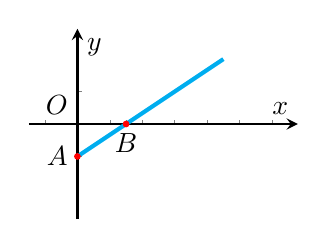
\begin{tikzpicture}[]
	\begin{axis}[
		width=5cm, height=4cm,
		axis lines=middle,
		xlabel=$x$, ylabel=$y$,
		xmin=-1.5, xmax=6.8, ymin=-1.5, ymax=1.5,
		xtick={-1,1,2,3,4,5,6},
		ytick={-1,1},
		xticklabel=\empty,
		yticklabel=\empty,
		extra x ticks={1.5},extra x tick labels={$B$},
		extra y ticks={-1},extra y tick labels={$A$},
		axis equal,
		tick align=inside, 
		tickwidth=1.5pt,%
		axis line style={thick},%
%		grid=major, grid style={gray!15},
		]
		\addplot[line width=1.5pt,cyan,domain=0:4.5,samples=2] {2/3*x-1};
		\addplot[only marks,mark=*,mark options={red},mark size=1pt]  coordinates {(0,-1)(1.5,0)};
		\node[above left] at (0,0){$O$};
	\end{axis}
\end{tikzpicture}
\captionof{figure}{}
\end{minipage}
\hspace{1em}
\begin{minipage}{0.3\textwidth}
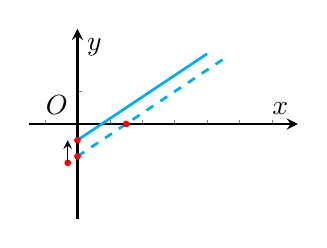
\begin{tikzpicture}[]
	\begin{axis}[
		width=5cm, height=4cm,
		axis lines=middle,
		xlabel=$x$, ylabel=$y$,
		xmin=-1.5, xmax=6.8, ymin=-1.5, ymax=1.5,
		xtick={-1,1,2,3,4,5,6},
		ytick={-1,1},
		xticklabel=\empty,
		yticklabel=\empty,
%		extra x ticks={1.5},extra x tick labels={B},
%		extra y ticks={-1},extra y tick labels={A},
		axis equal,
		tick align=inside, 
		tickwidth=1.5pt,%
		axis line style={thick},%
		%		grid=major, grid style={gray!15},
		]
		\addplot[line width=1pt,cyan,domain=0:4.5,samples=2,dashed] {2/3*x-1};
		\addplot[line width=1pt,cyan,domain=0:4,samples=2,] {2/3*x-0.5};
		\addplot[only marks,mark=*,mark options={red},mark size=1pt]  coordinates {(0,-1)(0,-0.5)(1.5,0)};
		\draw[fill=red,draw=red,->] (-0.3,-1.2) circle(1pt);
		\draw[-stealth] (-0.3,-1.2) -- (-0.3,-0.5);
		\node[above left] at (0,0){$O$};
	\end{axis}
\end{tikzpicture}
\captionof{figure}{}
\end{minipage}
\hspace{1em}
\begin{minipage}{0.3\textwidth}
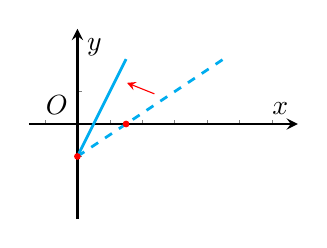
\begin{tikzpicture}[]
	\begin{axis}[
		width=5cm, height=4cm,
		axis lines=middle,
		xlabel=$x$, ylabel=$y$,
		xmin=-1.5, xmax=6.8, ymin=-1.5, ymax=1.5,
		xtick={-1,1,2,3,4,5,6},
		ytick={-1,1},
		xticklabel=\empty,
		yticklabel=\empty,
		%		extra x ticks={1.5},extra x tick labels={B},
		%		extra y ticks={-1},extra y tick labels={A},
		axis equal,
		tick align=inside, 
		tickwidth=1.5pt,%
		axis line style={thick},%
		%		grid=major, grid style={gray!15},
		]
		\addplot[line width=1pt,cyan,domain=0:4.5,samples=2,dashed] {2/3*x-1}node[pos=0.6](a){};
		\addplot[line width=1pt,cyan,domain=0:1.5,samples=2,] {2*x-1}node[pos=0.8](b){};
		\draw [-stealth,red](a) -- (b);
		\node[above left] at (0,0){$O$};
		\addplot[only marks,mark=*,mark options={red},mark size=1pt]  coordinates {(0,-1)(1.5,0)};
	\end{axis}
\end{tikzpicture}
\captionof{figure}{}
\end{minipage}
\end{center}

\end{frame}

\begin{frame}[t]{第4题 解答}
\begin{tcolorbox}[colback=orange!10,colframe=orange,title=\textbf{解}]
(1) 点 $A$：乘客量为 $0$ 时的收支差额（负值），即固定成本（亏损额）；

点 $B$：收支差额为 $0$ 的点，即盈亏平衡点，乘客量达到该点时不亏不盈；

射线 $AB$ 上的点：乘客量大于 $B$ 点对应值时，收支差额为正，线路开始盈利，乘客越多盈利越多。

\vspace{0.8em}
(2) 图(2)：射线平行上移（斜率不变），纵轴截距变大（$A$ 点上移），即 \alert{提高票价}，在相同乘客量下增加收入，使盈亏平衡点左移；

\vspace{0.3em}
图(3)：射线斜率变大（更陡），纵轴截距不变，即 \alert{降低成本}（如节约开支），保持票价不变而减少固定亏损，使收支随乘客量增长更快。
\end{tcolorbox}
\end{frame}

% ========== 第5题 ==========
\begin{frame}[t]{第5题：弹簧伸长与拉力}
\textbf{5.} 下表是拉力 $F$（单位：N）与弹簧伸长长度 $x$（单位：cm）的相关数据：

\vspace{0.3em}
\begin{center}
\begin{tabular}{lccccc}
\toprule
$F$ & 1 & 2 & 3 & 4 & 5 \\
$x$ & 14.2 & 28.8 & 41.3 & 57.5 & 70.2 \\
\bottomrule
\end{tabular}
\end{center}

\vspace{0.3em}
描点画出弹簧伸长长度随拉力变化的图象，并写出一个能基本反映这一变化现象的函数解析式。
\end{frame}

\begin{frame}[t]{第5题 解答}
\begin{tcolorbox}[colback=orange!10,colframe=orange,title=\textbf{解}]
观察数据，$F$ 每增加 $1$ N，$x$ 约增加 $14$ cm，近似线性关系。设 $x=kF+b$。

\vspace{0.3em}
取首尾两点 $(1,14.2)$、$(5,70.2)$：
\[
k=\frac{70.2-14.2}{5-1}=\frac{56}{4}=14,\quad b=14.2-14=0.2.
\]

\vspace{0.3em}
故函数解析式约为
\[
\alert{x=14F+0.2}\quad (\text{cm}).
\]

\vspace{0.3em}
（符合胡克定律 $F=k(x-x_0)$，在弹性限度内弹簧伸长与拉力成正比。）
\end{tcolorbox}
\end{frame}

\begin{frame}[t]{第5题 图象}
\begin{center}
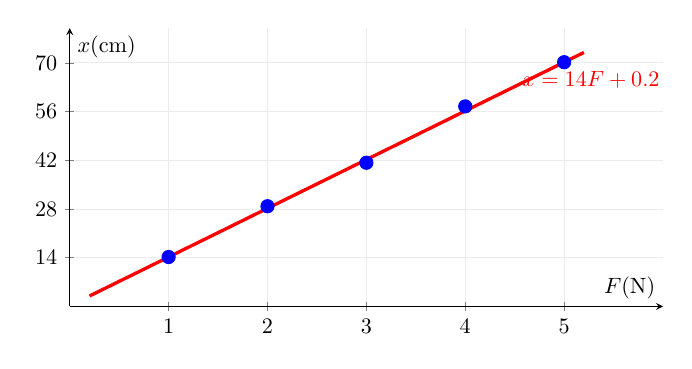
\begin{tikzpicture}[scale=0.8]
\begin{axis}[
    width=11cm, height=6cm,
    axis lines=middle,
    xlabel=$F$(N), ylabel=$x$(cm),
    xmin=0, xmax=6, ymin=0, ymax=80,
    xtick={1,2,3,4,5},
    ytick={14,28,42,56,70},
    grid=major, grid style={gray!15},
]
\addplot[only marks,mark=*,mark size=3pt,blue] coordinates {(1,14.2)(2,28.8)(3,41.3)(4,57.5)(5,70.2)};
\addplot[line width=1.5pt,red,domain=0.2:5.2,samples=2] {14*x+0.2};
\node[red,right] at (axis cs:4.5,65) {$x=14F+0.2$};
\end{axis}
\end{tikzpicture}
\end{center}
\end{frame}

\begin{frame}[c]
  \begin{center}
    {\Huge\calligra Thanks!}
  \end{center}
\end{frame}

\end{document}
